% Genere par src/figures_generator/figures_composition.py. Ne pas editer a la main.
\definecolor{centailment}{HTML}{0072B2}
\definecolor{cneutral}{HTML}{999999}
\definecolor{ccontradiction}{HTML}{D55E00}
\begin{figure}[t]
\centering
\tikzset{
  classentailment/.style={draw=centailment, line width=0.9pt, mark=none, const plot},
  classneutral/.style={draw=cneutral, line width=0.9pt, mark=none, const plot},
  classcontradiction/.style={draw=ccontradiction, line width=0.9pt, mark=none, const plot},
}
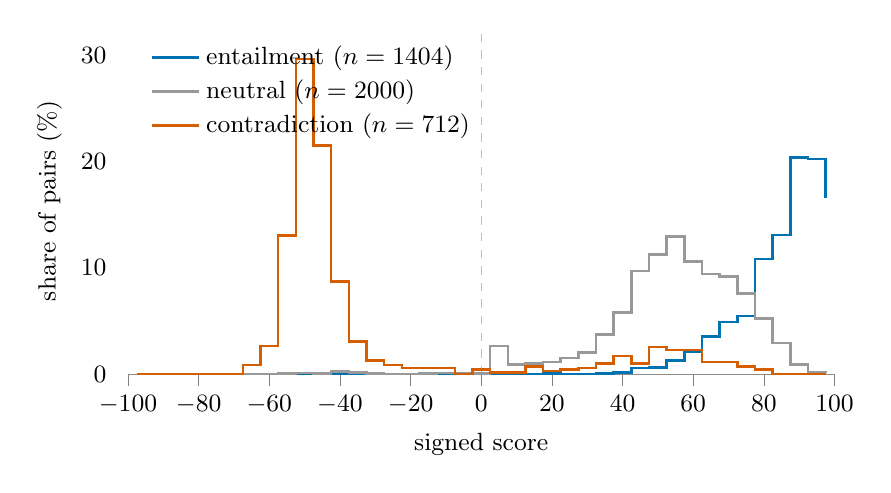
\begin{tikzpicture}
\begin{axis}[
  width=0.74\columnwidth, height=4.4cm, scale only axis,
  axis line style={draw=black!45, line width=0.3pt},
  axis x line*=bottom, axis y line*=left, y axis line style={draw=none},
  xmajorgrids=false, ymajorgrids=false, tick align=outside, ytick style={draw=none},
  xlabel={signed score}, ylabel={share of pairs (\%)},
  label style={font=\small}, tick label style={font=\small},
  xmin=-100, xmax=100, ymin=0,
  legend style={font=\small, draw=none, fill=none, at={(0.02,0.98)},
    anchor=north west, cells={anchor=west}},
]
\draw[draw=black!25, line width=0.3pt, dashed] (axis cs:0,0) -- (axis cs:0,\pgfkeysvalueof{/pgfplots/ymax});
\addplot[classentailment] coordinates {(-97.5,0.00) (-92.5,0.00) (-87.5,0.00) (-82.5,0.00) (-77.5,0.00) (-72.5,0.00) (-67.5,0.00) (-62.5,0.00) (-57.5,0.00) (-52.5,0.00) (-47.5,0.00) (-42.5,0.00) (-37.5,0.00) (-32.5,0.00) (-27.5,0.00) (-22.5,0.00) (-17.5,0.00) (-12.5,0.00) (-7.5,0.00) (-2.5,0.00) (2.5,0.07) (7.5,0.00) (12.5,0.00) (17.5,0.07) (22.5,0.00) (27.5,0.00) (32.5,0.07) (37.5,0.14) (42.5,0.57) (47.5,0.64) (52.5,1.28) (57.5,2.07) (62.5,3.56) (67.5,4.91) (72.5,5.48) (77.5,10.83) (82.5,13.11) (87.5,20.37) (92.5,20.23) (97.5,16.60)};
\addlegendentry{entailment ($n = 1404$)}
\addplot[classneutral] coordinates {(-97.5,0.00) (-92.5,0.00) (-87.5,0.00) (-82.5,0.00) (-77.5,0.00) (-72.5,0.00) (-67.5,0.00) (-62.5,0.00) (-57.5,0.05) (-52.5,0.10) (-47.5,0.05) (-42.5,0.25) (-37.5,0.15) (-32.5,0.05) (-27.5,0.00) (-22.5,0.00) (-17.5,0.05) (-12.5,0.10) (-7.5,0.05) (-2.5,0.05) (2.5,2.65) (7.5,0.90) (12.5,1.00) (17.5,1.15) (22.5,1.50) (27.5,2.05) (32.5,3.75) (37.5,5.80) (42.5,9.70) (47.5,11.25) (52.5,12.95) (57.5,10.60) (62.5,9.40) (67.5,9.20) (72.5,7.60) (77.5,5.25) (82.5,2.95) (87.5,0.90) (92.5,0.20) (97.5,0.30)};
\addlegendentry{neutral ($n = 2000$)}
\addplot[classcontradiction] coordinates {(-97.5,0.00) (-92.5,0.00) (-87.5,0.00) (-82.5,0.00) (-77.5,0.00) (-72.5,0.00) (-67.5,0.84) (-62.5,2.67) (-57.5,13.06) (-52.5,29.63) (-47.5,21.49) (-42.5,8.71) (-37.5,3.09) (-32.5,1.26) (-27.5,0.84) (-22.5,0.56) (-17.5,0.56) (-12.5,0.56) (-7.5,0.00) (-2.5,0.42) (2.5,0.14) (7.5,0.14) (12.5,0.70) (17.5,0.28) (22.5,0.42) (27.5,0.56) (32.5,0.98) (37.5,1.69) (42.5,0.98) (47.5,2.53) (52.5,2.25) (57.5,2.25) (62.5,1.12) (67.5,1.12) (72.5,0.70) (77.5,0.42) (82.5,0.00) (87.5,0.00) (92.5,0.00) (97.5,0.00)};
\addlegendentry{contradiction ($n = 712$)}
\end{axis}
\end{tikzpicture}
\caption{Signed score by gold class on the SICK half of the test split, $\alpha = 2$, binned at width $5$. Contradictions concentrate near $-50$ and entailments near $+80$. SICK neutral pairs are related captions rather than unrelated sentences, so they belong near the middle of the positive half and not at zero; what matters is that the product does not drag them across it.}
\label{fig:distribution}
\end{figure}
